\documentclass[12pt]{article}

\usepackage[polish]{babel}
\usepackage{graphicx}
\usepackage{polski}
\usepackage[utf8]{inputenc}

\title{Raport z projektu SNR -- sieci głębokie w zastosowaniu do klasyfikacji obrazów zawierających numery budynków}
\author{
        Łukasz Neumann \\
            \and
        Witold Oleszkiewicz \\
}
\date{\today}

\begin{document}
\maketitle


\section{Wstęp}

Niniejszy raport przedstawia wyniki prac w ramach projektu z przedmiotu Sztuczne Sieci Neuronowe. Prezentujemy dane i oprogramowanie, które wykorzystaliśmy do zbudowania i przetrenowania głębokiej splotowej sieci neuronowej oraz wyniki walidacji tej sieci na zbiorze zdjęć cyfr oznaczających numery budynków. Dodatkowo zbadaliśmy wpływ użycia warstwy \textit{dropout} na jakość klasyfikacji.

\section{Dane}

Dane wykorzystane w danym projekcie są rzeczywistymi danymi, które pochodzą z obrazów Google Street View \cite{dane}. Na obrazach są widoczne tabliczki z numerami budynków. Wykorzystaliśmy zbiór po wstępnej obróbce, która polegała na znalezieniu na zdjęciach obszarów, na których widoczne są przede wszystkim cyfry składające się na numer budynku, których szerokość i wysokość są większe niż połowa szerokości i wysokości analizowanych zdjęć.

Każde ze zdjęć jest kolorowe oraz składa się z 32x32 pikseli. Do każdego ze zdjęć jest przyporządkowana etykieta, która ozacza cyfrę widoczną na zdjęciu (od 0 do 9). Wykorzystaliśmy dwa dostępne zbiory:

\begin{itemize}
\item zbiór trenujący, który składa się z 73257 zdjęć cyfr,
\item zbiór testujący, która składa się z 26032 zdjęć cyfr.
\end{itemize}

\section{Oprogramowanie}

Do budowania i trenowania głębokich sieci neuronowych zastosowaliśmy Keras \cite{keras} -- bibliotekę/API wysokiego poziomu w języku Python oraz bibliotekę Theano \cite{theano}, z której nie korzystaliśmy bezpośrednio, a posłużyła ona jako \textit{backend}. 

\section{Przygotowanie danych}

Zdjęcia skonwertowano z kolorowych na czarno-białe, gdyż kolor nie wpływa na klasyfikację cyfry.

Zamiast etykiet (od 0 do 9) dla każdego ze zdjęć, zastosowaliśmy wektor składający się z dziewięciu zera i jednej jedynki, która znajduje się na $i$-tej pozycji dla cyfry $i$.

\section{Architektura sieci głębokich i dodatkowy problem badawczy}

Zdefiniowaliśmy sieć neuronową składającą się z 12 warstw ukrytych (w tym 4 warstw splotowych):

\begin{tabular}{|r|c|c|c|}
  \hline 
  Warstwa & Wymiary wyjścia & Liczba parametrów & Opis\\
  \hline
  conv 2D & 30x30x32 & 320 & 32 maski 3x3\\
  \hline
  dropout & 30x30x32 &  & usunięcie 20\% neuronów \\
  \hline
  conv 2D & 28x28x32 & 9248 & 32 maski 3x3\\
  \hline
  max pool 2D & 14x14x32 &  & okno 2x2\\
  \hline
  conv 2D & 12x12x32 & 9248 & 32 maski 3x3\\
  \hline
  dropout & 12x12x32 &  & usunięcie 20\% neuronów \\
  \hline
  conv 2D & 10x10x32 & 9248 & 32 maski 3x3\\
  \hline
  max pool 2D & 5x5x32 &  & okno 2x2\\
  \hline
  flatten & 800 &  & \\
  \hline
  dense & 512 & 410112 & \\
  \hline
  dropout & 512 &  & usunięcie 50\% neuronów \\
  \hline
  dense & 10 & 5130 & \\
  \hline

\end{tabular} 

Jako funkcję aktywacji neuronów użyto funkcję ReLU: $a(x) = \max(0, x)$. Wartość normy wag została ograniczona do $3$. W warstwie wyjściowej zastosowano funkcję \textit{softmax}: $\sigma(z)_j=\frac{\exp{z_j}}{\sum_k \exp(z_k)}$.

Do optymalizacji sieci neuronowej wybrano algorytm stochastycznego spadku gradientu z parametrami momentum:$0.9$, decay:$0.0004$, learning rate:$0.04$. Optymalizację przeprowadzano przez 100 epok, gradient obliczano na podsatwie 128 zdjęć ze zbioru trenującego. Zastosowano funkcję celu, entropia krzyżowa: $y\log a + (1-y)\log(1-a)$, gdzie $a$ to wartość wyjścia a $y$ to oczekiwana wartość wyjścia.

Dodatkowym problemem badawczym było przeanalizowanie wyników walidacji powyższej sieci neuronowej z usuniętymi warstwami \textit{dropout}.

\section{Wyniki}

\begin{figure}[!h]
\centering
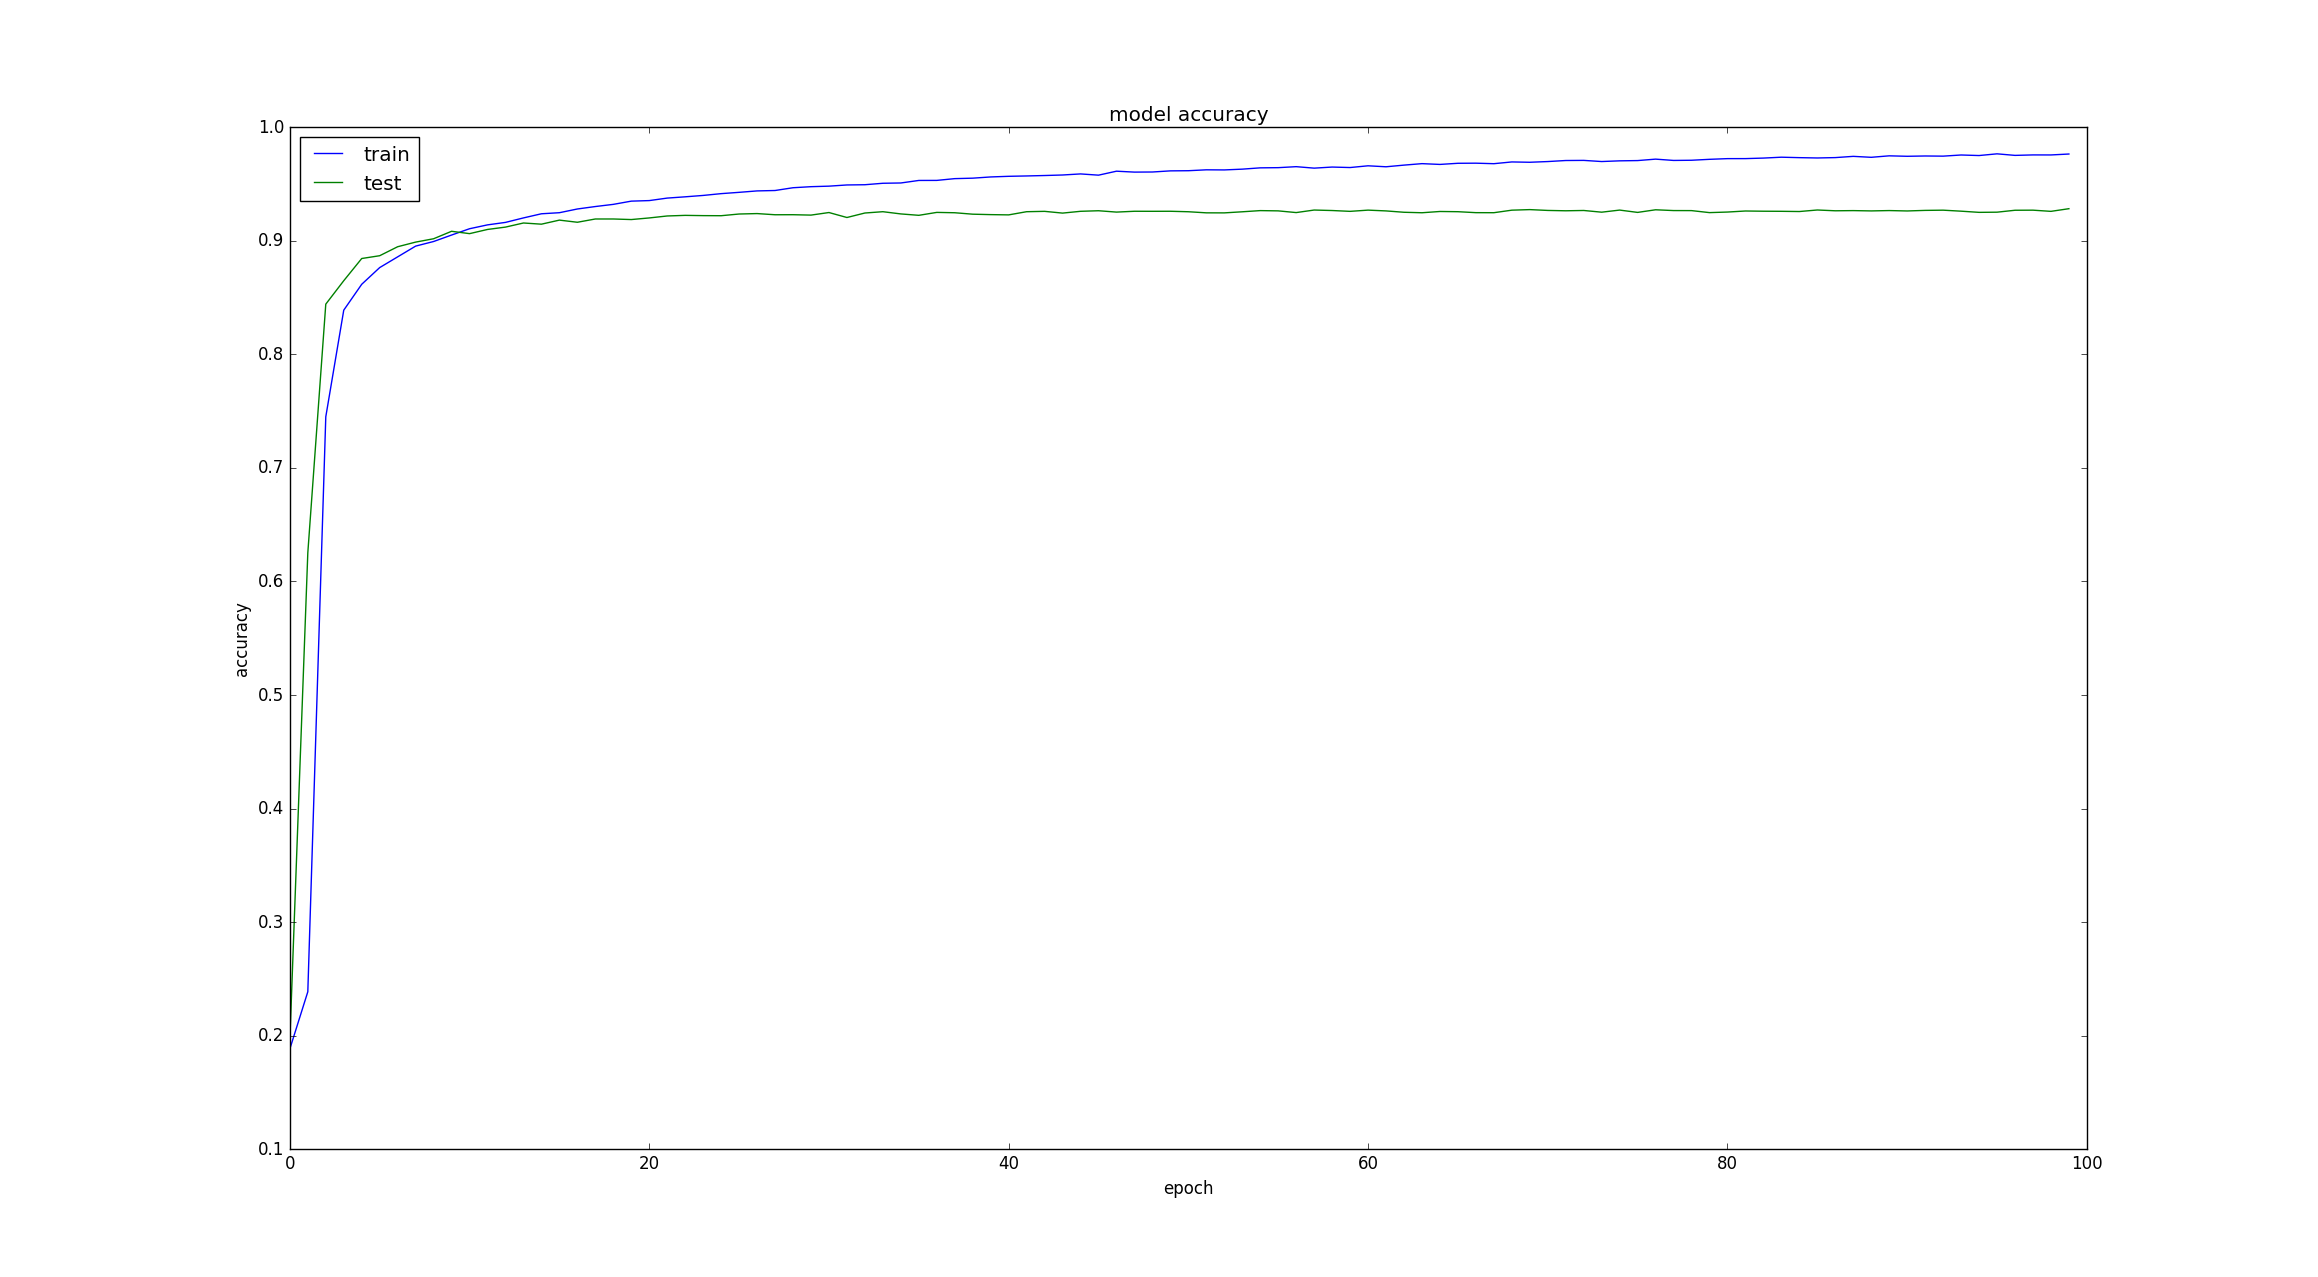
\includegraphics[scale=0.25]{acc_dropout}
\caption{Dokładność klasyfikacji dla sieci neuronowej z \textit{dropoutem}.}
\end{figure}

\begin{figure}[!h]
\centering
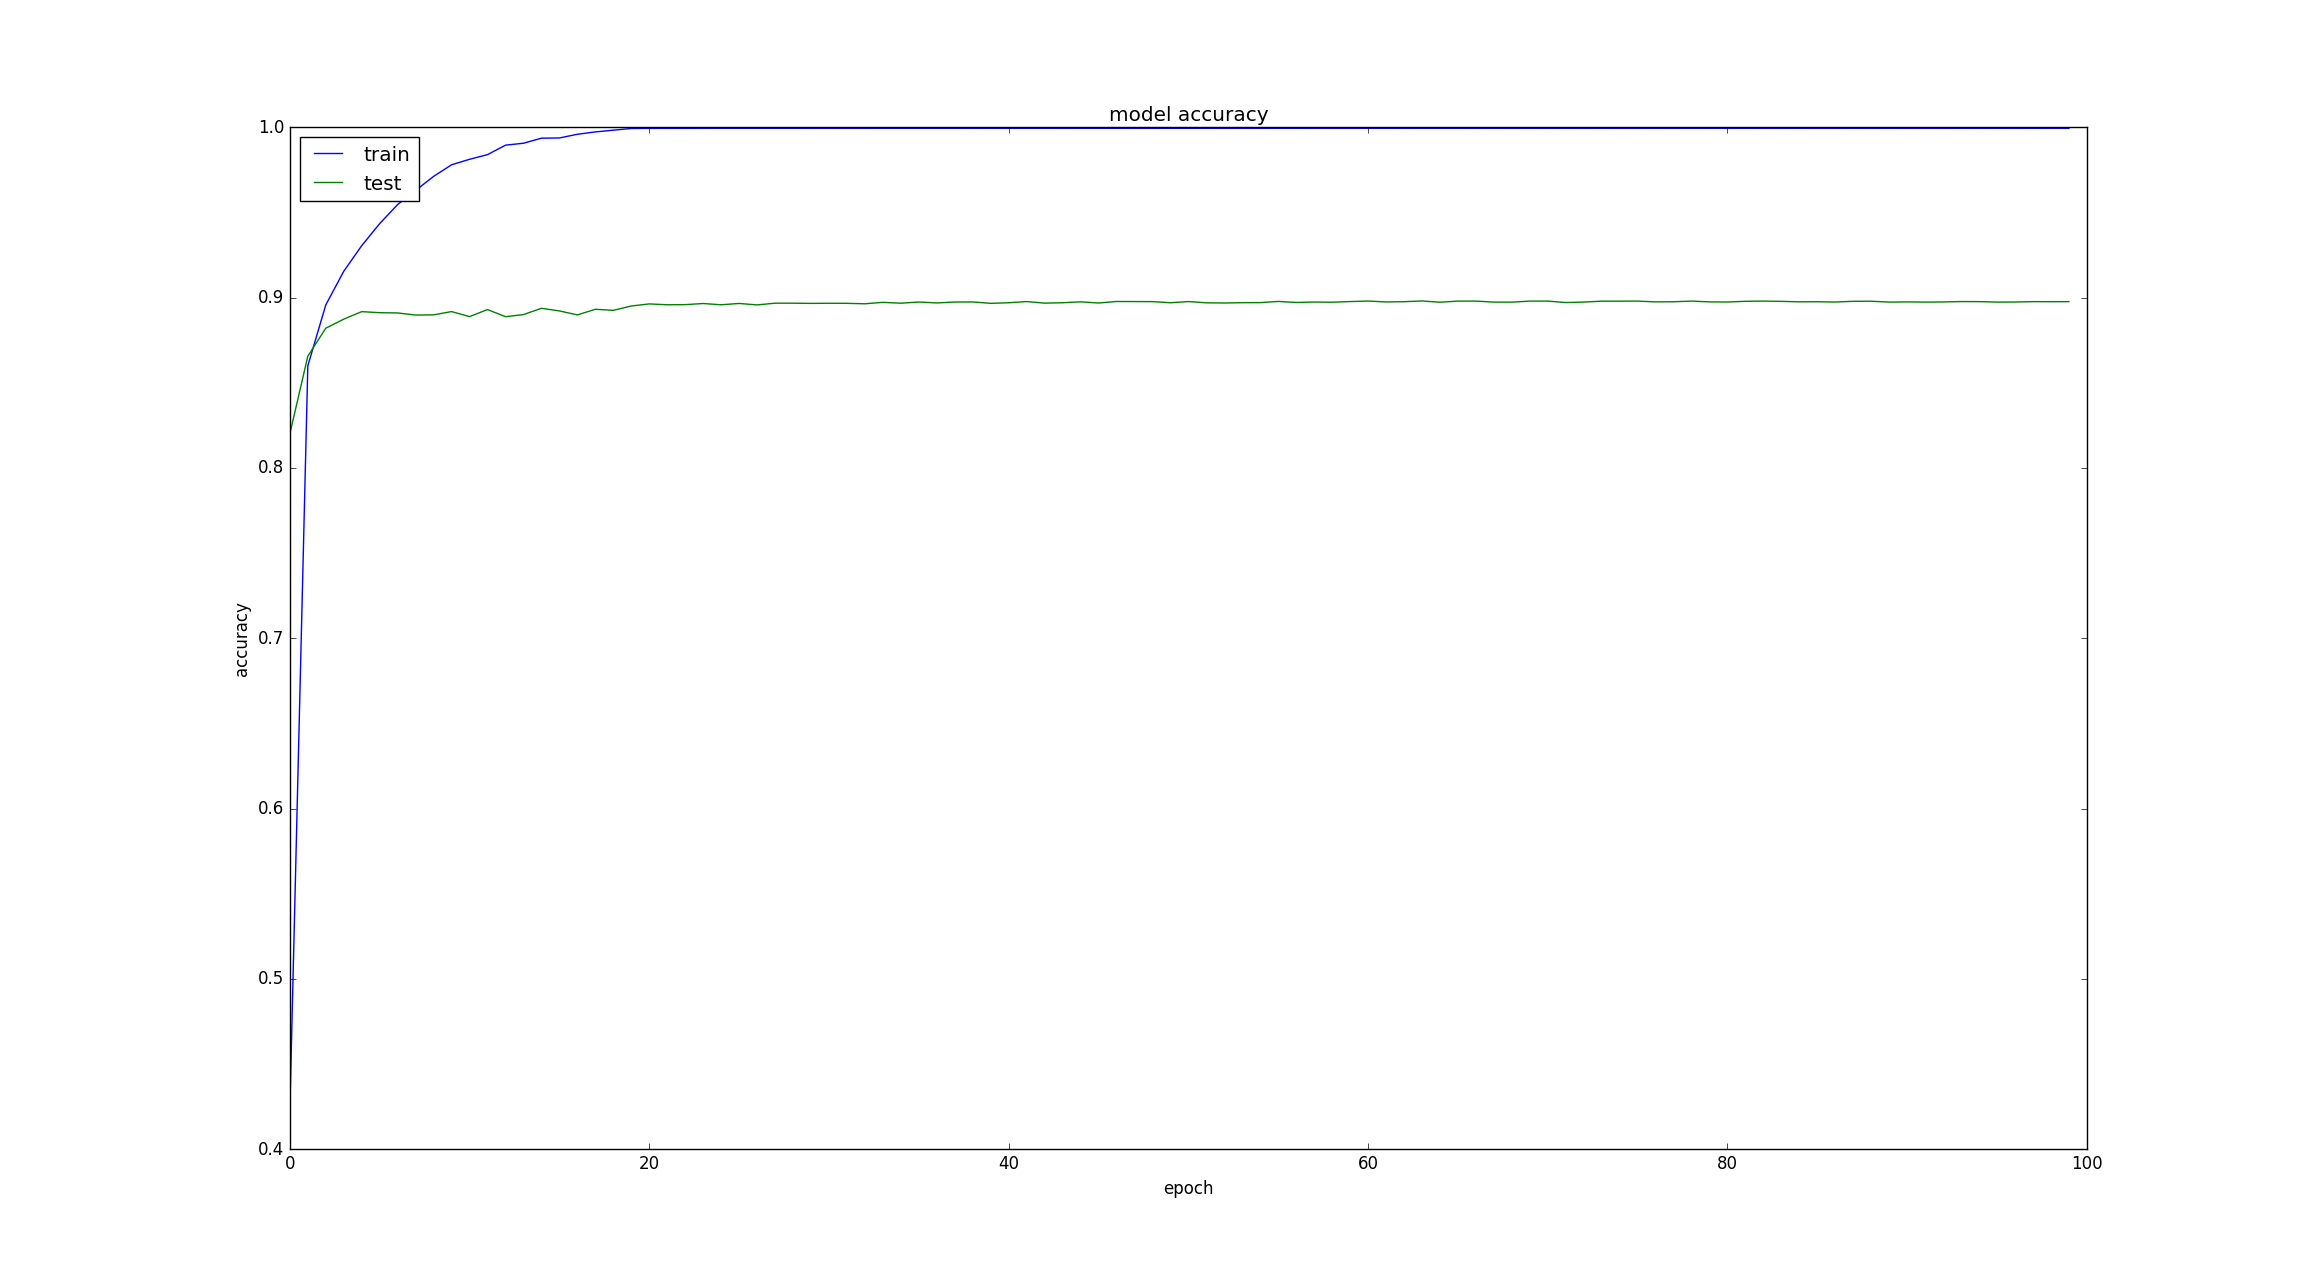
\includegraphics[scale=0.25]{acc_no_dropout}
\caption{Dokładność klasyfikacji dla sieci neuronowej bez \textit{dropoutu}.}
\end{figure}

\begin{figure}[!h]
\centering
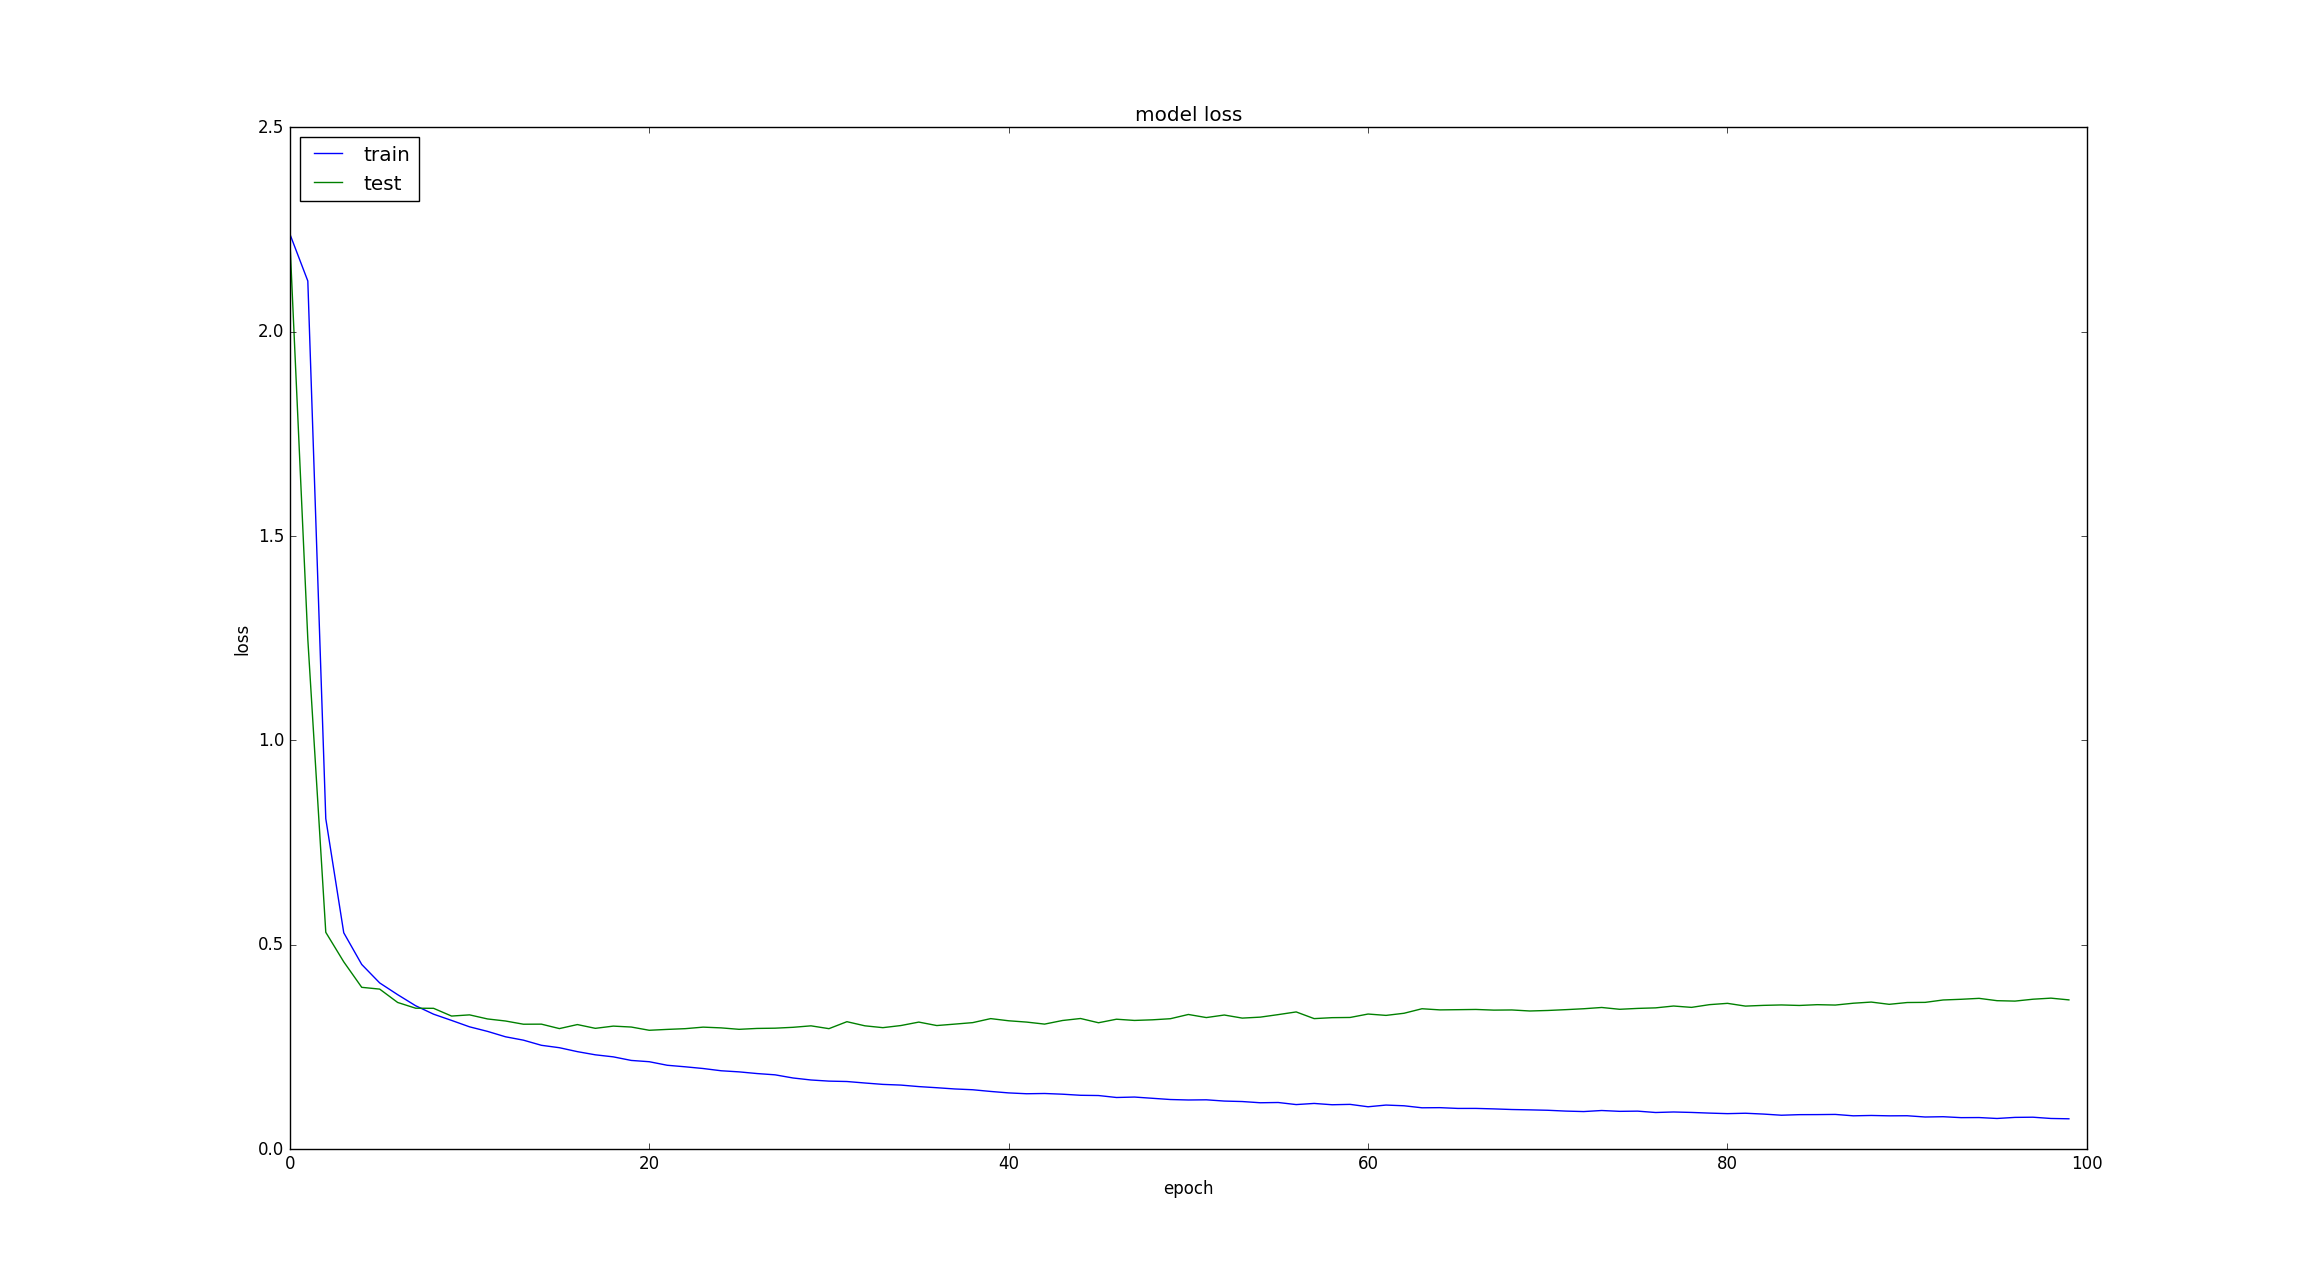
\includegraphics[scale=0.25]{loss_dropout}
\caption{Funkcja celu dla głębokiej sieci neuronowej z \textit{dropoutem}.}
\end{figure}

\begin{figure}[!h]
\centering
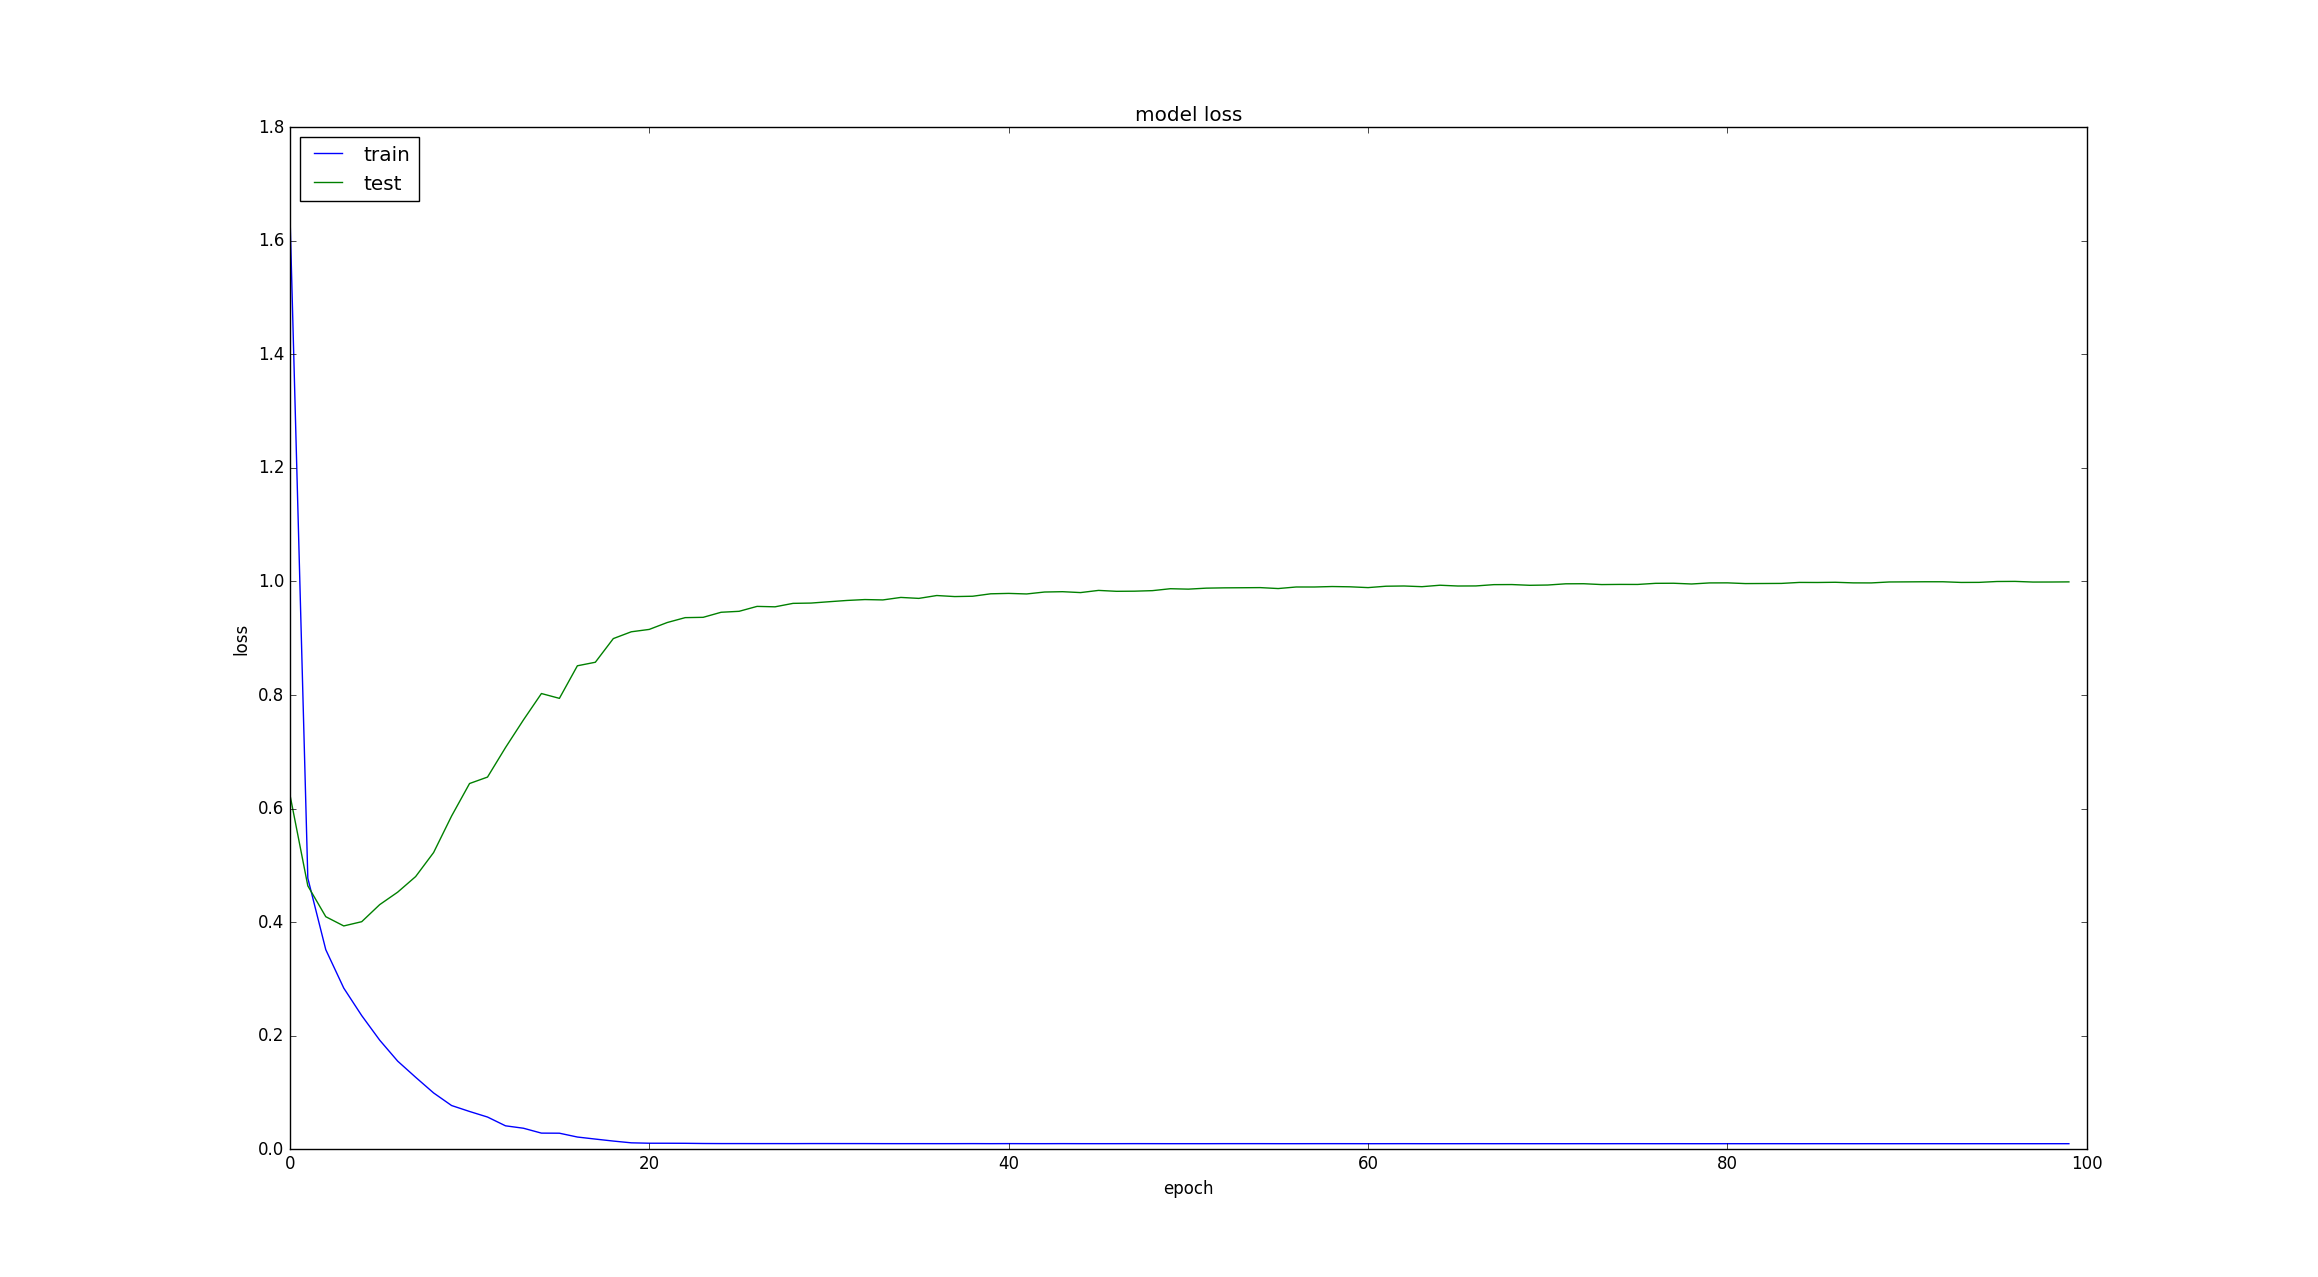
\includegraphics[scale=0.25]{loss_no_dropout}
\caption{Funkcja celu dla głębokiej sieci neuronowej bez \textit{dropoutu}.}
\end{figure}

TODO: opis wyników

\begin{thebibliography}{9}

\bibitem{dane}
The Street View House Numbers (SVHN) Dataset,
Yuval Netzer, Tao Wang, Adam Coates, Alessandro Bissacco, Bo Wu, Andrew Y. Ng
Reading Digits in Natural Images with Unsupervised Feature Learning NIPS Workshop on Deep Learning and Unsupervised Feature Learning
2011
http://ufldl.stanford.edu/housenumbers/

\bibitem{keras}
https://keras.io

\bibitem{theano}
http://deeplearning.net/software/theano/
\end{thebibliography}{9}

\end{document}
